\section{Proactive Approaches}
\label{sec:proactive}
Sun \emph{et al.} \cite{sun2015raptor} recently demonstrated a successful real-world BGP routing attack on a Tor guard relay by announcing a more-specific prefix (i.e., /24 prefix against /23 prefix), which covers the guard relay. We have shown in Section \ref{hijack_interception_measurement} that network-level adversaries can hijack a portion of the traffic by announcing an equally-specific prefix (i.e., same prefix length). To counter these two routing attacks, we propose two methods, respectively: 1) convincing relay operators to move the relay into a /24 prefix to defend against a more-specific prefix attack, and 2) introducing a new Tor guard relay selection algorithm that minimizes the likelihood that a Tor client sees a hijacked route in the case of an equally-specific prefix attack.

\subsection{Using /24 Prefixes}
\label{subsec:24prefix}
Network-level adversaries can hijack internet traffic by announcing a more-specific prefix that belongs to the true origin AS. Since BGP routing prefers longer prefixes over shorter ones, the traffic will go to the false origin with the more-specific prefix instead. The longest prefix length that BGP usually accepts is /24, and thus any prefix that's shorter than /24 is vulnerable to more-specific prefix attacks. Sun \emph{et al.} \cite{sun2015raptor} recently found that more than 90\% of BGP prefixes hosting relays are
shorter than /24, making them vulnerable to a more-specific BGP prefix attack. 

%We measured the distribution of prefix lengths in relation to Tor bandwidth using the Tor consensus data in January 2016; this is shown in ~\ref{fig_prefixlen}. Consistent with the findings in \cite{sun2015raptor}, a large percentage of the bandwidth are under prefixes shorter than /24. 

%\begin{figure}[ht!]
%\centering
%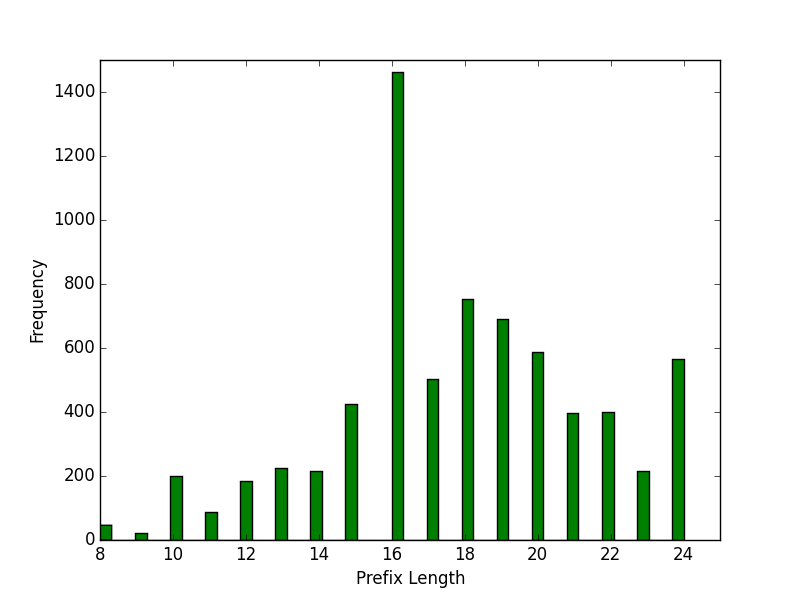
\includegraphics[width=80mm]{prefix_len_graph}
%\caption{Distribution of Tor bandwidth to Prefix Lengths \yixin{we need to fix this plot} \label{fig_prefixlen}}
%\end{figure}

Therefore, one way to defend against more-specific prefix hijack attacks is to move Tor guard relays into /24 prefixes. One concern that may arise is the extra burden which can be created on the routing table if announcing /24 prefixes for all Tor guard relays. We obtained a snapshot of the routing table from RouteViews ~\cite{routeviews}, and the Tor consensus data from January 2016. We found that there are 607,335 unique prefixes in the routing table, whereas there are only 1484 unique /24 prefixes covering all Tor guard relays (roughly 0.24\% of the routing table prefixes). Thus, the impact on the routing table size would be negligible. 

To make real world impact of this approach, we start a campaign in progress by contacting Tor relay operators, and suggesting that they move their Tor relays into /24 prefixes. We start with cooperating with an anonymous Tor relay operator, which contains a Tor relay under a /16 prefix. The approach they took was to announce an additional /24 prefix that covers the Tor relay, while still maintaining the original /16 announcement. This minimized the amount of work needed to move Tor relays into /24 prefixes. 

\subsection{Guard Relay Selection}
\label{subsec:relayselection}

Guard relays are at an important position in the Tor circuit, since they have direct connections with Tor clients. Section ~\ref{subsec:24prefix} discusses how to mitigate more-specific prefix hijack attacks; however, even if the guard relay belongs to a /24 prefix, it is still subject to an equally-specific prefix hijack attack. We have shown in Section \ref{hijack_interception_measurement} that high-bandwidth Tor relays could belong to ASes with low resilience to prefix hijack attacks, which put many Tor users at risk. Therefore, we propose a new guard relay selection algorithm that incorporates AS resilience in order to mitigate such active prefix hijacks on Tor.

%It has been shown that network-level adversaries can launch a more-specific BGP prefix attack to hijack the Tor traffic from the guard relay to the malicious AS \cite{sun2015raptor}. This can be potentially prevented by advertising /24 prefixes, as discussed in Section ~\ref{subsec:24prefix}. However, even if the guard relay belongs to a /24 prefix, it is still subject to an equally-specific prefix attack. Unlike more-specific attacks which spread through the whole internet, equally-specific attacks can only affect connections within a small range - i.e., ASes that have more preferred paths to the hijacking AS than the true origin AS. Thus, picking a Tor guard relay that has relatively high AS resiliency against such equally-specific attacks could protect Tor clients from being affected and deanonymized by network-level adversaries. Therefore, we propose a new guard relay selection algorithm that incorporates this aspect.

\subsubsection{Design Goals}
\begin{enumerate}
\item \emph{Mitigate prefix hijacks on Tor.} This is the main goal of the new guard relay selection algorithm. The algorithm computes the AS resilience against prefix hijacks of all Tor guard relays from the client source AS, and prefers the ones that have higher resilience, minimizing the likelihood that the client would be affected by a prefix hijack on its guard relay. 
\item \emph{Protect the anonymity of Tor clients.} In addition to lowering possibilities of being hijacked, the algorithm should also protect the anonymity of Tor users by balancing preferences among relays and providing rigorously assessed anonymity bounds. 
\item \emph{Performance and Load balancing.} The algorithm should incorporate relay bandwidth into the selection decision and avoid causing excessive traffic congestion on low bandwidth relays.
%\item \emph{Performance overhead.} The algorithm should have a reasonable performance overhead over the vanilla Tor algorithm when bootstrapping, and fast page load time. 
\end{enumerate}

\subsubsection{Mitigate Prefix Hijacks on Tor}

In Section \ref{hijack_methodology}, we measured AS resilience of each Tor-related AS based on the metrics proposed by~\cite{lad2007understanding}. The algorithm computes \emph{total} resilience of an AS by summing individual resiliencies from each source AS. \emph{However, the Tor client would only care about the individual resilience to a Tor-related AS from the source AS where the client is located}. Thus, instead of computing the total resilience, we use Algorithm ~\ref{algo:calcres} to calculate resilience $R(i)$ of each Tor-related AS $i$, from the client AS $t$. 

Tor relay selection is bandwidth-aware and prefers high bandwidth relays. The probability of each relay $i$ being chosen is based on its bandwidth $B(i)$. Thus, in order to still provide clients with the load balancing option of Tor bandwidths, we offer a tunable parameter $\alpha$ in the relay selection algorithm combining AS resiliency $R(i)$ and bandwidth $B(i)$. Each relay $i$ will be assigned a weight as following:
\begin{equation*}
W(i) = \alpha \times R(i) + (1 - \alpha) \times B(i)
\end{equation*}
Note that, when $\alpha$ is set to $0$, the relay selection becomes the same as bandwidth-only selection; while when $\alpha$ is set to $1$, the selection becomes resiliency-only selection. 

\subsubsection{Randomization is needed}
\label{relay_randomization}
If we simply select the set of guard relays based on the probability of $W(i)/\sum W(i)$, an adversary can potentially run a relay that has an AS-level path with high local preferences and/or short path length to the Tor client, such that it has high resilience from the client AS as the source. And it therefore obtains a high probability of being chosen. Furthermore, the Tor client might also be susceptible to fingerprinting attacks due to the differences in relay selection probabilities based on the AS-location of the client. An adversary that can observe the client for a long enough time may be able to infer the AS-location of the client based on its observed relay selection choices. Thus, we need to take into account these potential vulnerabilities and protect the anonymity of clients. Note that the weight of a Tor relay depends on two components: (1) the resilience of the AS in which the relay is located, and (2) the relay's bandwidth. The relay's bandwidth is not specific to client locations, and thus would not reveal any client identities; in addition, due to resource constraints, it is not trivial to run a relay with significantly higher bandwidth than all other relays to obtain high probability of being chosen. While on the contrary, AS resilience of relays \emph{is} client-specific, and requires much fewer resources to run a malicious relay with high AS resilience.

Instead of using resilience $R(i)$ for relay $i$ directly in the weight calculation, we first adjust it to $R(i)\prime$ by calculating the estimated inclusion probability of the relay in a random sampling of size $(g \cdot N)$ using the algorithm proposed by Tille ~\cite{tille1996elimination}. Note that $N$ corresponds to the total number of ASes containing Tor guard relays, and $g$ is a configurable parameter indicating the percentage of random sampling we want to perform. The steps are as following:
\begin{enumerate}
\item For each relay $i$, $R(i)\prime = \frac {k \cdot R(i)} {\sum R(i)}$ in which $k$ is initially equal to the sample size $(g \cdot N)$.
\item For each relay $i$, if $R(i)\prime > 1$, $R(i)\prime = 1$ and $k = k - 1$.
\item Repeat the above process until each $R(i)\prime$ is in $[0,1]$.
\item For each relay $i$, $R(i)\prime = \frac{R(i)\prime} {g \cdot N}$
\end{enumerate}

%performing a pseudorandom sampling without replacement using algorithm proposed by Tille (cite here). We compute the inclusion probability of each relay $i$ into a sample of size $(g \cdot total\_TorASes)$ given the fraction of its resilience $R(i)$ over total resiliences $\sum R(i)$, and then divide the inclusion probability by sample size $(g \cdot total\_TorASes)$ to get the probability of being chosen randomly within the sample. So the new resilience weight becomes:
%
%\begin{equation*}
%R(i) \prime = \frac {\pi(i | (g \cdot N))} {g \cdot N}
%\end{equation*}
%
%in which $\pi(i | m)$ represents inclusion probability of relay $i$ given sample size $m$, and $N$ is the total number of ASes that Tor relays reside in. $g$ is a configurable parameter indicating the percentage of random sampling we want to perform in the Tor-related AS set. 

Note that when $g$ is set to $0$, then no random sampling will be performed, while if $g$ is set to $1$, then all relays will have the same $R(i)\prime$ in their weights. 

%Instead of selecting relay directly based on its weight, we will first select a cluster of 
%\begin{equation*}
%m + \alpha \cdot g \cdot (N - m)
%\end{equation*}
%number of relays, in which $m$ is the minimum number of relays needed (i.e., 1 for single guard and 3 for multiple guards), $N$ is the total number of relays and $g$ is a configurable parameter indicating the maximum percentage of additional relays we want to pick into the cluster. Then, we will pick the guard relay(s) at random from the cluster. Note that when $g$ is set to $0$, then no additional randomization will be performed, while if $g$ is set to $1$, all guard relays will be picked randomly regardless of bandwidth or resiliency. We will evaluate how different values of $g$ may impact the security and anonymity.

\subsubsection{Implementation on Tor}
Mapping the IP addresses of the Tor client and Tor relays to their respective AS is necessary before we can compute AS resilience. In order to preserve the anonymity of the Tor client and not reveal its location to outside servers or anyone who can observe it's communications, the client will perform the IP to ASN mapping locally by utilizing the Maxmind ASN database ~\cite{maxmind}, which can be included in the Tor download package. Note that the vanilla Tor client uses the Maxmind GeoIP database for IP to Country mapping, which is already included in the Tor package as well. In addition, the client will use the AS topology database from CAIDA \cite{caida} for AS-level path inference in the resilience calculation. 

If the Tor client specifies in the torrc configuration file that the AS resilience-aware guard relay selection is preferred, and supplies an $\alpha$ value as the tunable parameter, the following procedure will be invoked:

\begin{enumerate}
\item If the Maxmind ASN file and AS topology file have not been downloaded, the Tor client will download the two files from Maxmind and CAIDA, respectively, and save them in the local data directory. 
\item The Tor client will perform IP to ASN mapping, and compute the AS resilience $R(i)$ of all candidate relays from the client AS as the source AS. 
\item The Tor client will perform random sampling on all ASes containing candidate relays and adjust the resilience value to $R(i)\prime$.
\item The Tor client will compute a weight for each candidate relay using formula $W(i) = \alpha \times R(i) \prime + (1 - \alpha) \times B(i)$. 
%\item The Tor client will select a cluster of $m + \alpha \cdot g \cdot (N - m)$ relays based on their weights, and then randomly select the guard relay(s) from the cluster. 
\item The Tor client will proceed with the path selection. The remaining part of the circuit construction process stays the same as it is in Tor. 
\end{enumerate}

\subsection{Security and Anonymity Evaluation}
We evaluate the security and anonymity of the Tor guard relay selection algorithm from three perspectives: (1) reduction in probability of a Tor client being affected by a hijack attack on the Tor guard relay, (2) balancing preferences in relay selection to avoid favoring certain relays significantly more than the others, (3) vulnerability to client fingerprinting attacks, and (4) rigorously assessed anonymity bound for a given Tor client. 

\subsubsection{Probability of a Tor client being affected by a hijack attack on Tor guard relay}
\label{attack_probability}
This is the main goal of the new relay selection algorithm. Let $P_{pick}(i)$ denotes the probability that a Tor client will choose relay $i$ using our algorithm, and $P_{deceived}(i)$ denotes the probability that a Tor client will be deceived if relay $i$ is being hijacked. $P_{deceived}(i)$ can be calculated using similar method in Section ~\ref{hijack_interception_measurement}, the details of which will be addressed in the Appendix. The overall probability of a Tor client being affected by a hijack attack on guard relay can then be expressed as:
\begin{equation*}
\sum_{i \in \{all guard relays\}} P_{pick}(i) * P_{deceived}(i)
\end{equation*}

We first evaluate the probability without random sampling for five values of $\alpha=\{0, 0.25, 0.5, 0.75, 1\}$ with $1000$ randomly selected ASes as the source AS and Tor consensus data from January 2016. Figure ~\ref{fig_attack} shows the result. Table ~\ref{tbl_attack_reduction} shows the average percentage of reduction in the probability of being affected by a hijack attack compared to $\alpha=0$. We can see that $\alpha=1$ has the lowest probability of being affected by an attack, with an average of 31\% reduction. 

\begin{figure}[ht!]
\centering
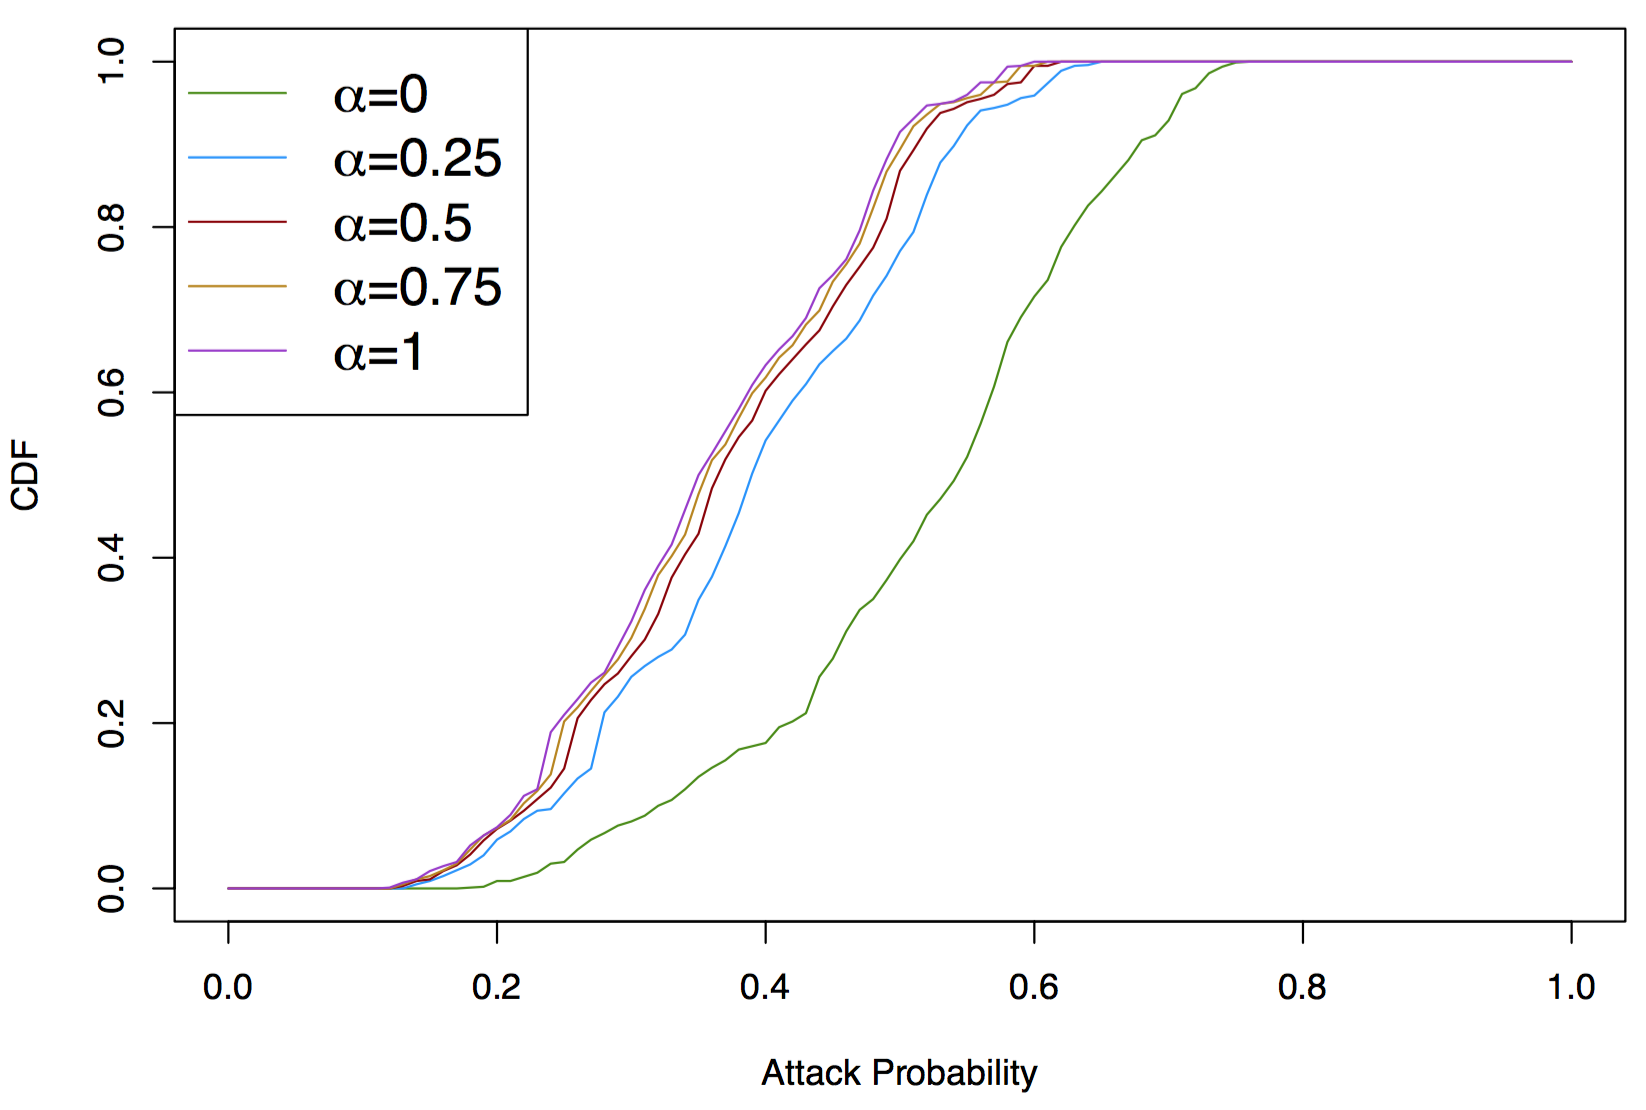
\includegraphics[width=80mm]{figure/attack}
\caption{Attack Probability with different $\alpha$ values \label{fig_attack}}
\end{figure}

%in probability for the $1000$ client ASes compared to $\alpha=0$. When $\alpha=0.25$, the probability increases a bit, with an average of 24\% reduction compared to $\alpha=0$. While $\alpha=\{0.5,0.75\}$ has similar probability to $\alpha=1$, with average of 28\% and 30\% reduction in probability, respectively. 

We then evaluate it with random sampling of $g=10\%$. Figure ~\ref{fig_attack_random} shows the comparison of $\alpha=\{0.25, 0.5\}$ with and without random sampling. Table ~\ref{tbl_attack_reduction} shows the average percentage of reduction in attack probability with $g=10\%$ random sampling. We can see that there is only a very slight decrease in the reduction percentage with the random sampling. 

\begin{figure}[ht!]
\centering
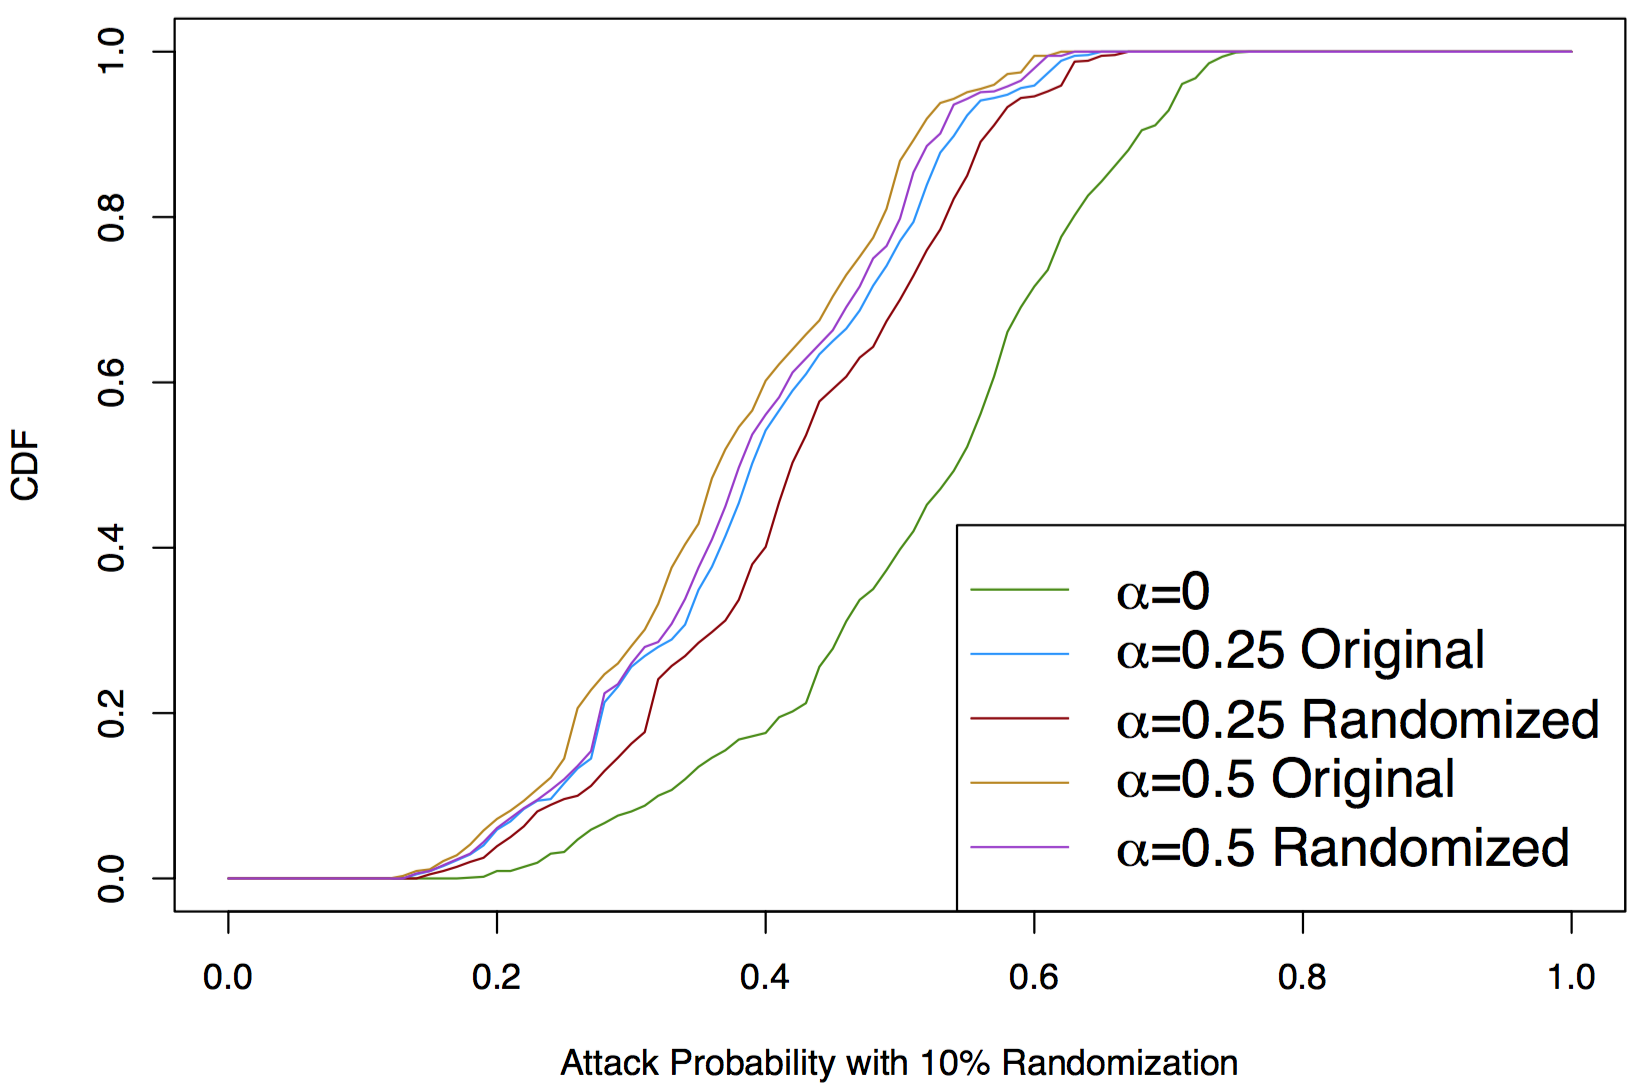
\includegraphics[width=80mm]{figure/attack_randomize}
\caption{Attack Probability with $g=10\%$ sampling \label{fig_attack_random}}
\end{figure}

\begin{table}[ht!]
\begin{center}
 \begin{tabular}{ p{5mm} | p{2.5cm} | p{2.5cm}}
    \hline
    $\alpha$ & Without Random Sampling & With  $g=10\%$ sampling\\ \hline
    0.25 & 24\% & 19\% \\
    0.5 & 28\% & 25\% \\
    0.75 & 30\% & 29\% \\
    1 & 31\% & 31\% \\
    \hline
  \end{tabular}
\end{center}
\caption{Percentage of reduction in attack probability compared to $\alpha=0$ \label{tbl_attack_reduction}}
\end{table}

\subsubsection{Balancing Relay Selection Preferences} 
We want to main good balance among the weights/preferences for each candidate relay to avoid strongly favoring certain relays over the others. For instance, for a given Tor client, if relay $i$ has 90\% probability of being chosen while all other relays totals up to 10\% probability, then this can create potential security vulnerabilities, let alone performance issues. An adversary may easily target relay $i$ to launch an attack, or even manipulate the selection algorithm to strongly favor a relay run by the adversary. Thus, we want to evaluate the variance in probabilities of a given Tor client picking any particular relay and show that it's well-balanced. 

We used Gini coefficient as the variance evaluation metric, as it has been used in previous work ~\cite{akhoondi2012lastor}. We first evaluate without random sampling, for five values of $\alpha: \{0, 0.25, 0.5, 0.75, 1\}$ with $1000$ randomly selected ASes as source AS and Tor consensus data from January 2016. Figure ~\ref{fig_gini} shows the result. The green line to the right is when $\alpha = 0$, which is solely based on bandwidth, resulting in a Gini coefficient of $0.51$ for all source ASes. The Gini coefficients for the other four $\alpha$ values which involve resilience-based selection are much lower than bandwidth-only selection, meaning that there is lower skew in probability of selecting any particular relay and thus is more well-balanced. 

\begin{figure}[ht!]
\centering
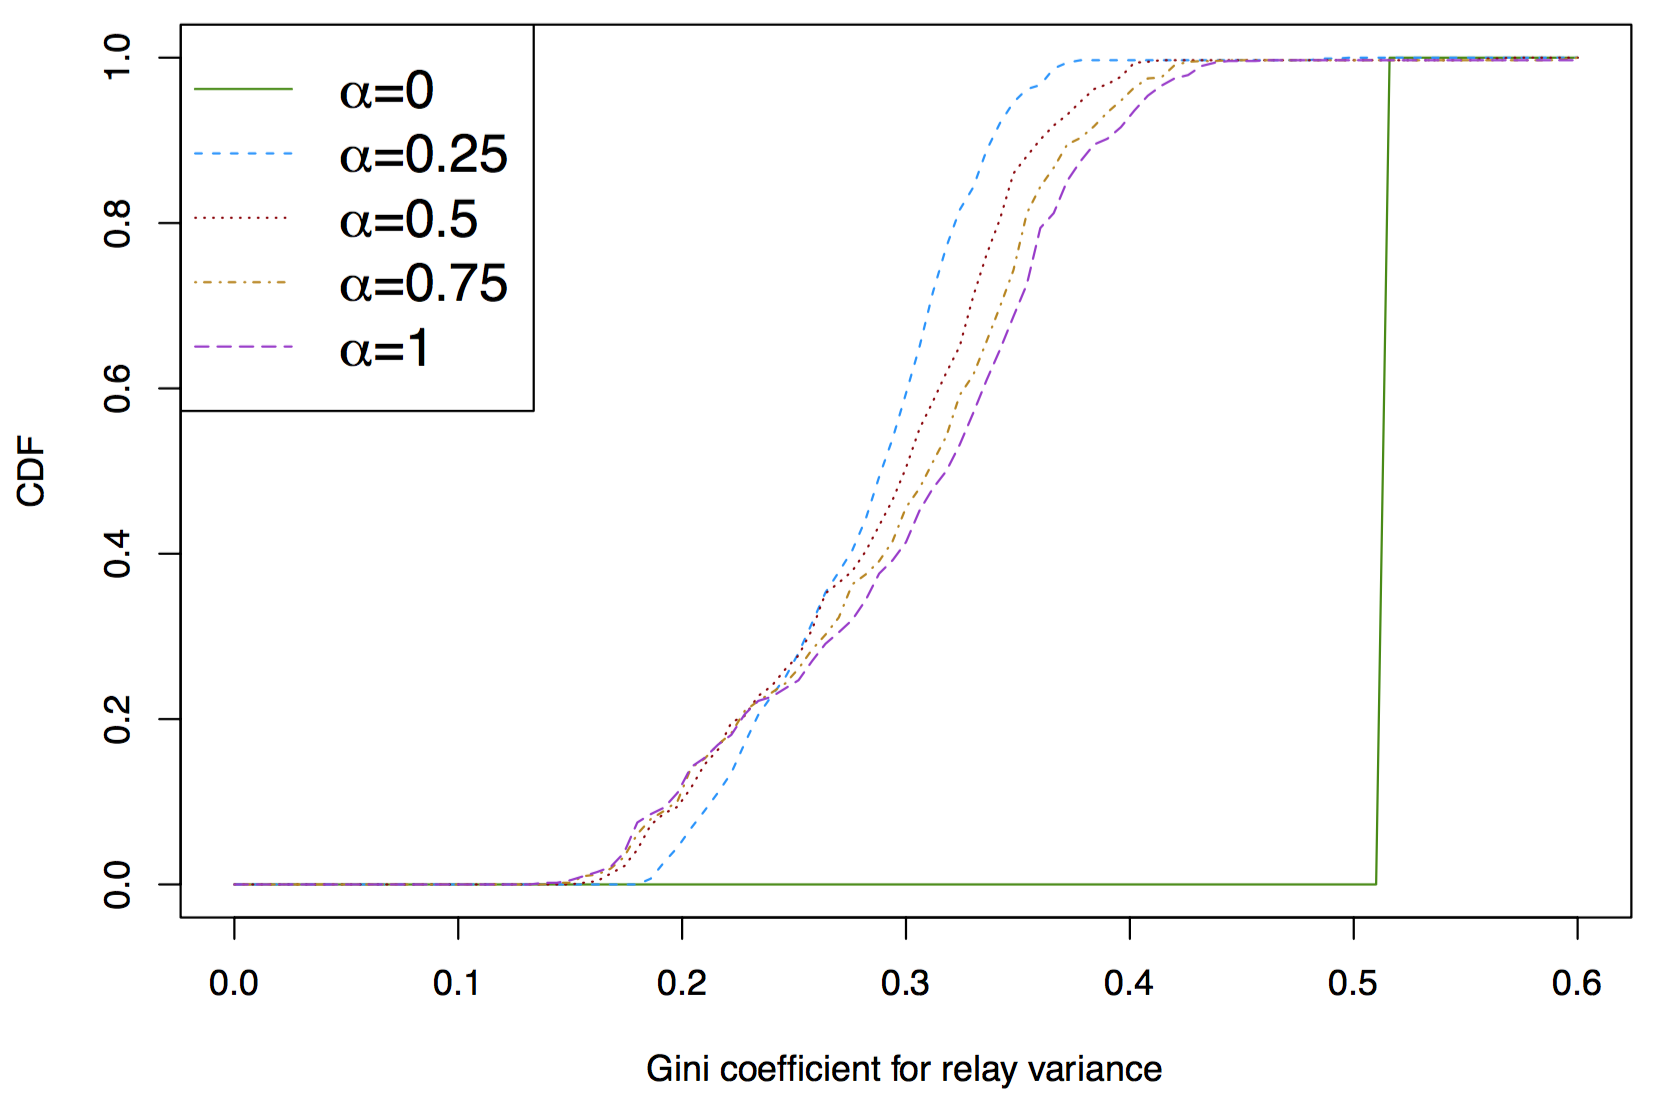
\includegraphics[width=80mm]{figure/gini_relay_variance}
\caption{Gini coefficients for variance in relay selection preferences given a Tor client. Lower Gini coefficient value indicates higher variance and less skew. \label{fig_gini}}
\end{figure}

\subsubsection{Vulnerability to client fingerprinting attacks}
This is a potential security tradeoff of the relay selection algorithm. We briefly discussed in Section ~\ref{relay_randomization} about fingerprinting a client location based on its preferences of relays in the long term. For instance, for a given relay, if client $a$ has 70\% probability of choosing the relay while client $b$ only has 30\% probability, then an adversary can observe the client's choice of relays overtime to infer client information. The resilience component of our relay selection algorithm may be subjective to such fingerprinting attacks, which we will evaluate here. 

We used Gini coefficient again as the variance evaluation metric, but evaluating \emph{the variance in the probability of each client choosing a given relay} instead. Figure ~\ref{fig_gini_client} shows the result for $1000$ randomly selected ASes as client AS. 

We can see that the bandwidth-only selection in Vanilla Tor ($\alpha = 0$) has perfect Gini coefficient value of 0 for all relays, since given a relay, the probability of it being chosen is the same across all clients. With resilience-based selection, the skews in probabilities are higher. When $\alpha = 1$ (resilience-only), $80\%$ of the relays have coefficients $> 0.4$. This skew in probability might be exploited by adversaries who can observe the client over a period of time to infer client locations given the differences in relay selection.

We then evaluate it again with $g=10\%$ random sampling. Note that since $\alpha=\{0.75,1\}$ does not have a significant advantage in attack resilience over $\alpha=\{0.25,0.5\}$ in Section ~\ref{attack_probability}, while resulting in higher skew in probabilities, so we focus on evaluating the later here. Figure ~\ref{fig_gini_client_random} shows that by performing $10\%$ random sampling, when $\alpha=0.25$, $80\%$ of the relays have coefficients reduced to $< 0.28$. Although this may still pose some vulnerability to client fingerprinting, we argue that since Tor clients only select guard relays at bootstrapping time, and would then use the same guard relays over several months or until the relays become unavailable, so fingerprinting the client could not be done in a reasonably short time, especially given the low variance of probabilities (although not perfect) as shown.


\begin{figure}[ht!]
\centering
\begin{subfigure}{.25\textwidth}
\centering
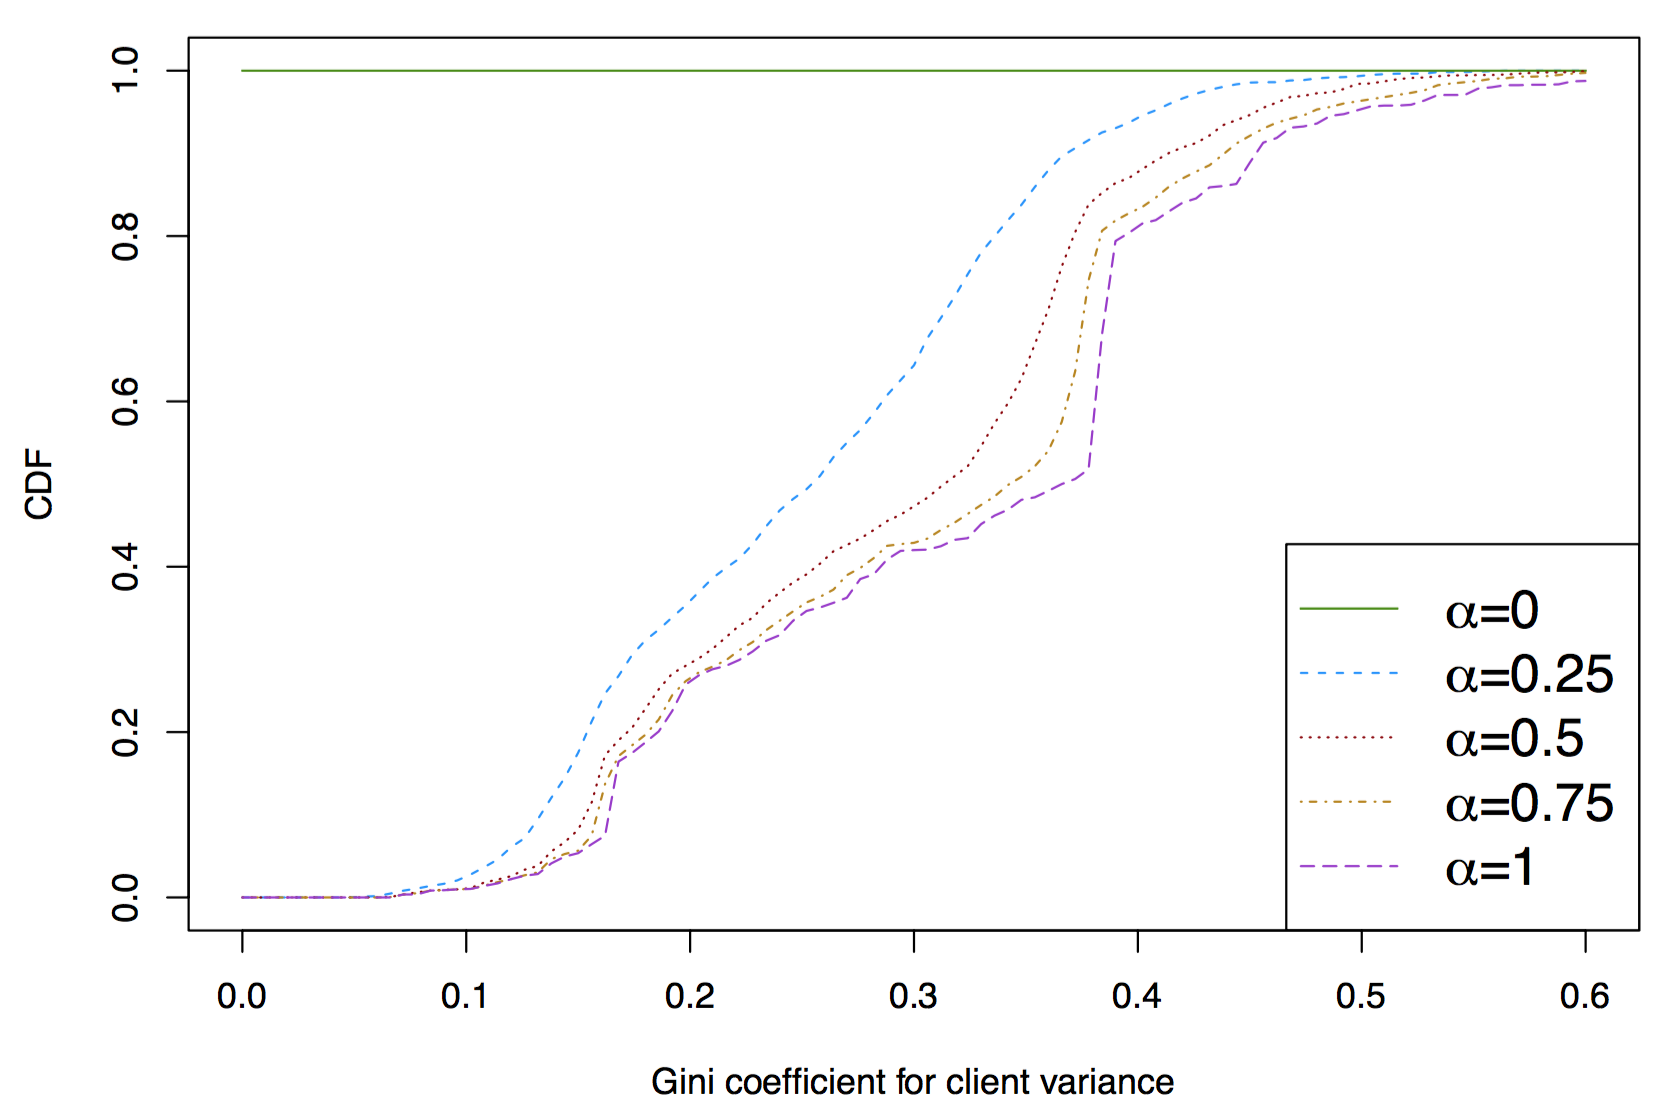
\includegraphics[width=.9\linewidth]{figure/gini_client_variance}
\caption{Without random sampling \label{fig_gini_client}}
\end{subfigure}%
\begin{subfigure}{.25\textwidth}
\centering
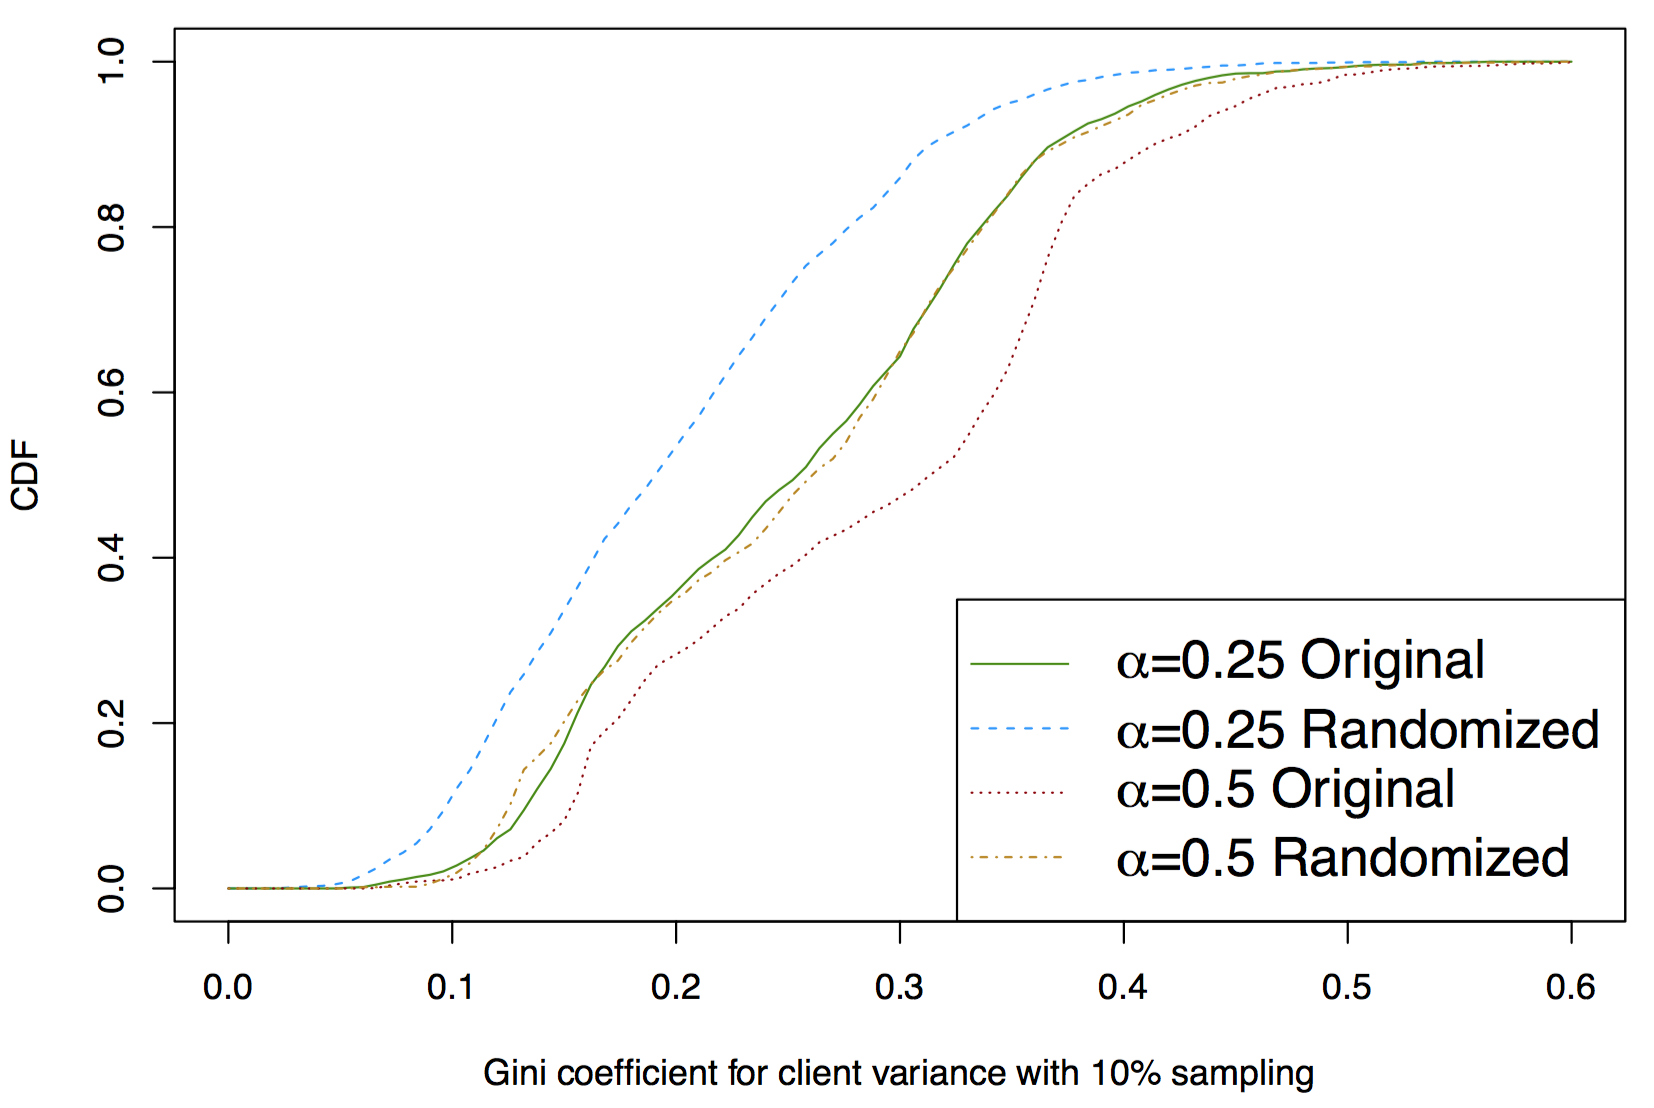
\includegraphics[width=.9\linewidth]{figure/randomize_client_gini}
\caption{With $g=10\%$ sampling \label{fig_gini_client_random}}
\end{subfigure}
\caption{Gini coefficients for variance in client's probability of choosing a given relay.}
\label{fig:gini_client}
\end{figure}

\subsubsection{Formal anonymity assessment}
Finally, we evaluate the anonymity of a given Tor client using MATor, a framework for assessing the degree of anonymity in Tor with rigorously proved anonymity bounds ~\cite{backes2014nothing}. We implemented our new relay selection algorithm into MATor source code, and evaluated it in comparison with vanilla Tor. Note that we picked the top Tor client location AS6128 ~\cite{juen2012protecting} to evaluate here. We used default configuration of multiplicative factor $\epsilon=1.3$, ports setting of HTTPS+IRC vs. HTTPS, and $0.5\%$ of total nodes as compromised nodes. We evaluated using Tor consensus files from 2/1/2016 - 2/9/2016 and server descriptor from February 2016. Figure ~\ref{fig_mator} shows the result. 

\begin{figure}[ht!]
\centering
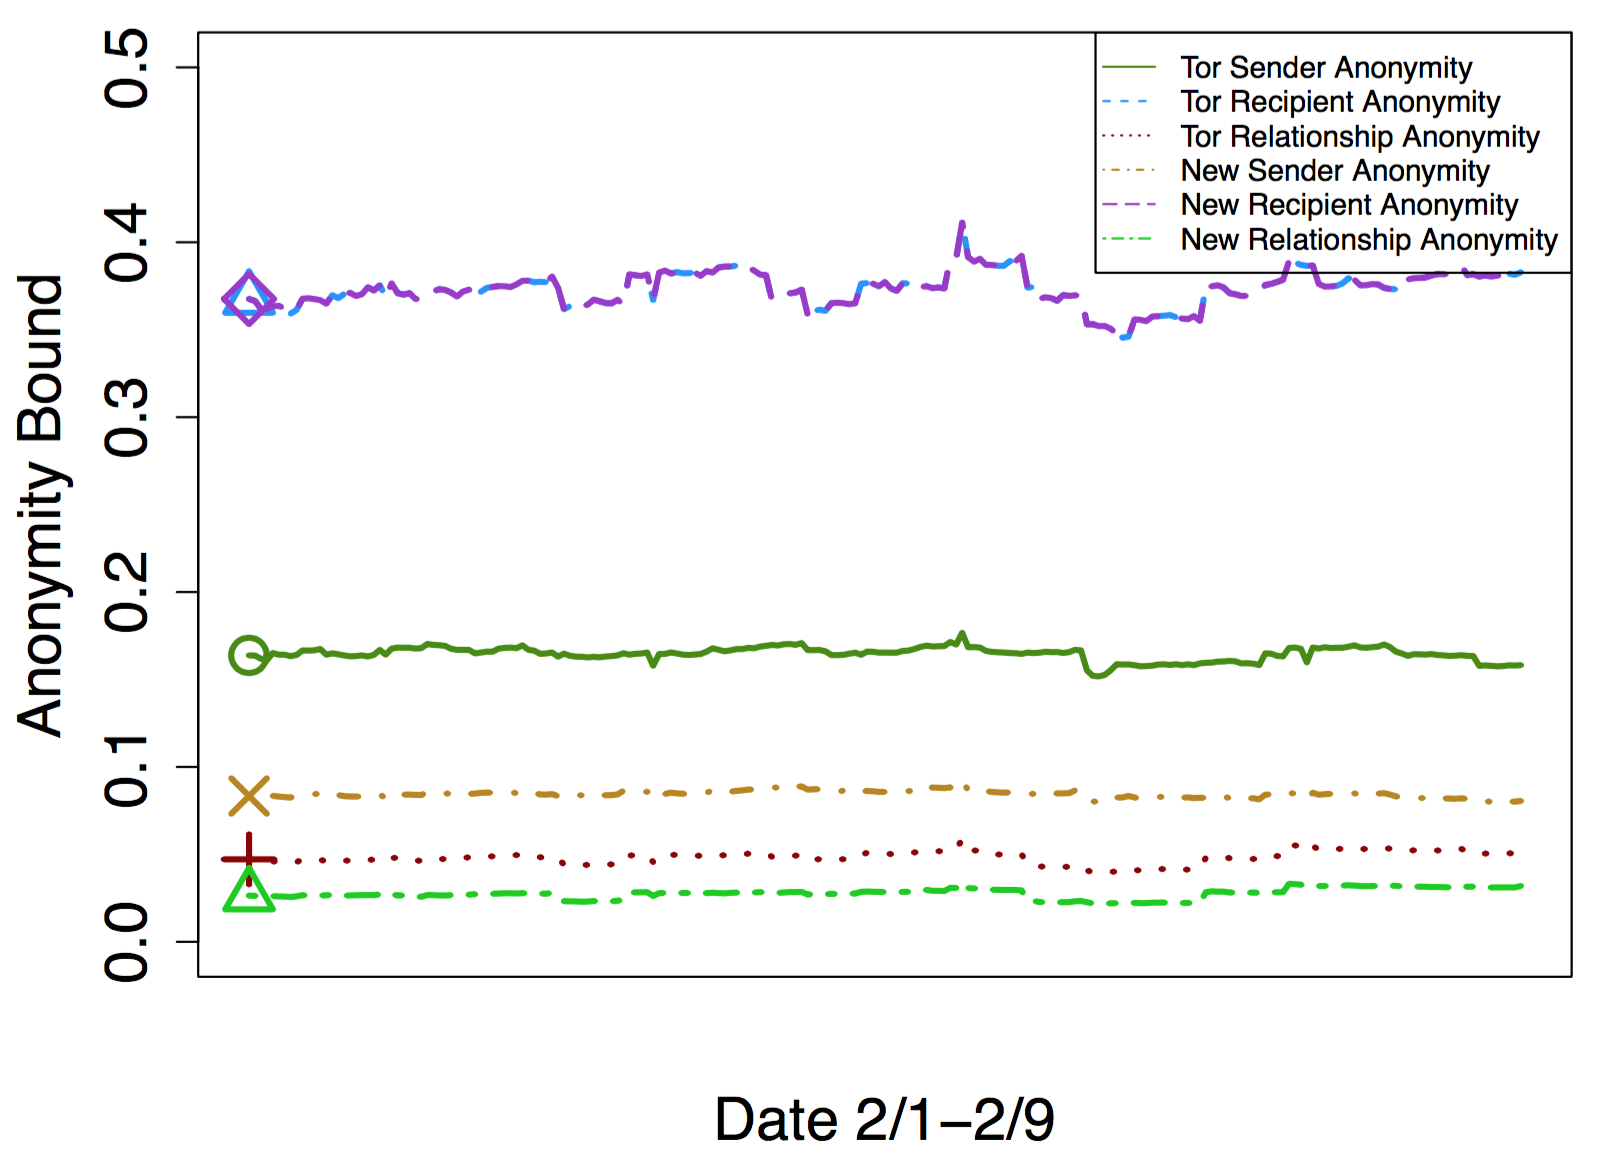
\includegraphics[width=80mm]{figure/mator}
\caption{MATor Anonymity Bound 2/1/2016 - 2/9/2016\label{fig_mator}}
\end{figure}

MATor evaluates three anonymity notions (sender, recipient, and relationship anonymity). The full details of the anonymity definitions are described in ~\cite{backes2014nothing}. The result shows that our new guard relay selection has tighter anonymity bounds on sender and relationship anonymities compared to current Tor path selection, indicating better anonymity guarantees. The recipient anonymity remains the same as vanilla Tor, which is expected since we do not alter selection algorithm for exit relays. 


%However, the variance in relay selection probability \emph{across} different source ASes is bigger than bandwidth-only: when $\alpha = 0$, all sources ASes have the same gini coefficient of $0.607$, while for other $\alpha$ values, the gini coefficient could vary from approximately $0.2$ to $0.4$, depending on the source AS. 


\subsection{Performance Evaluation}

We first evaluate the runtime of the AS resilience calculation given a source AS. We pick $1000$ ASes randomly as the source AS, and record how much time it takes each of them to complete the calculation. Most of the source ASes finish within $0.6$ second. \\

%\begin{figure}[ht!]
%\centering
%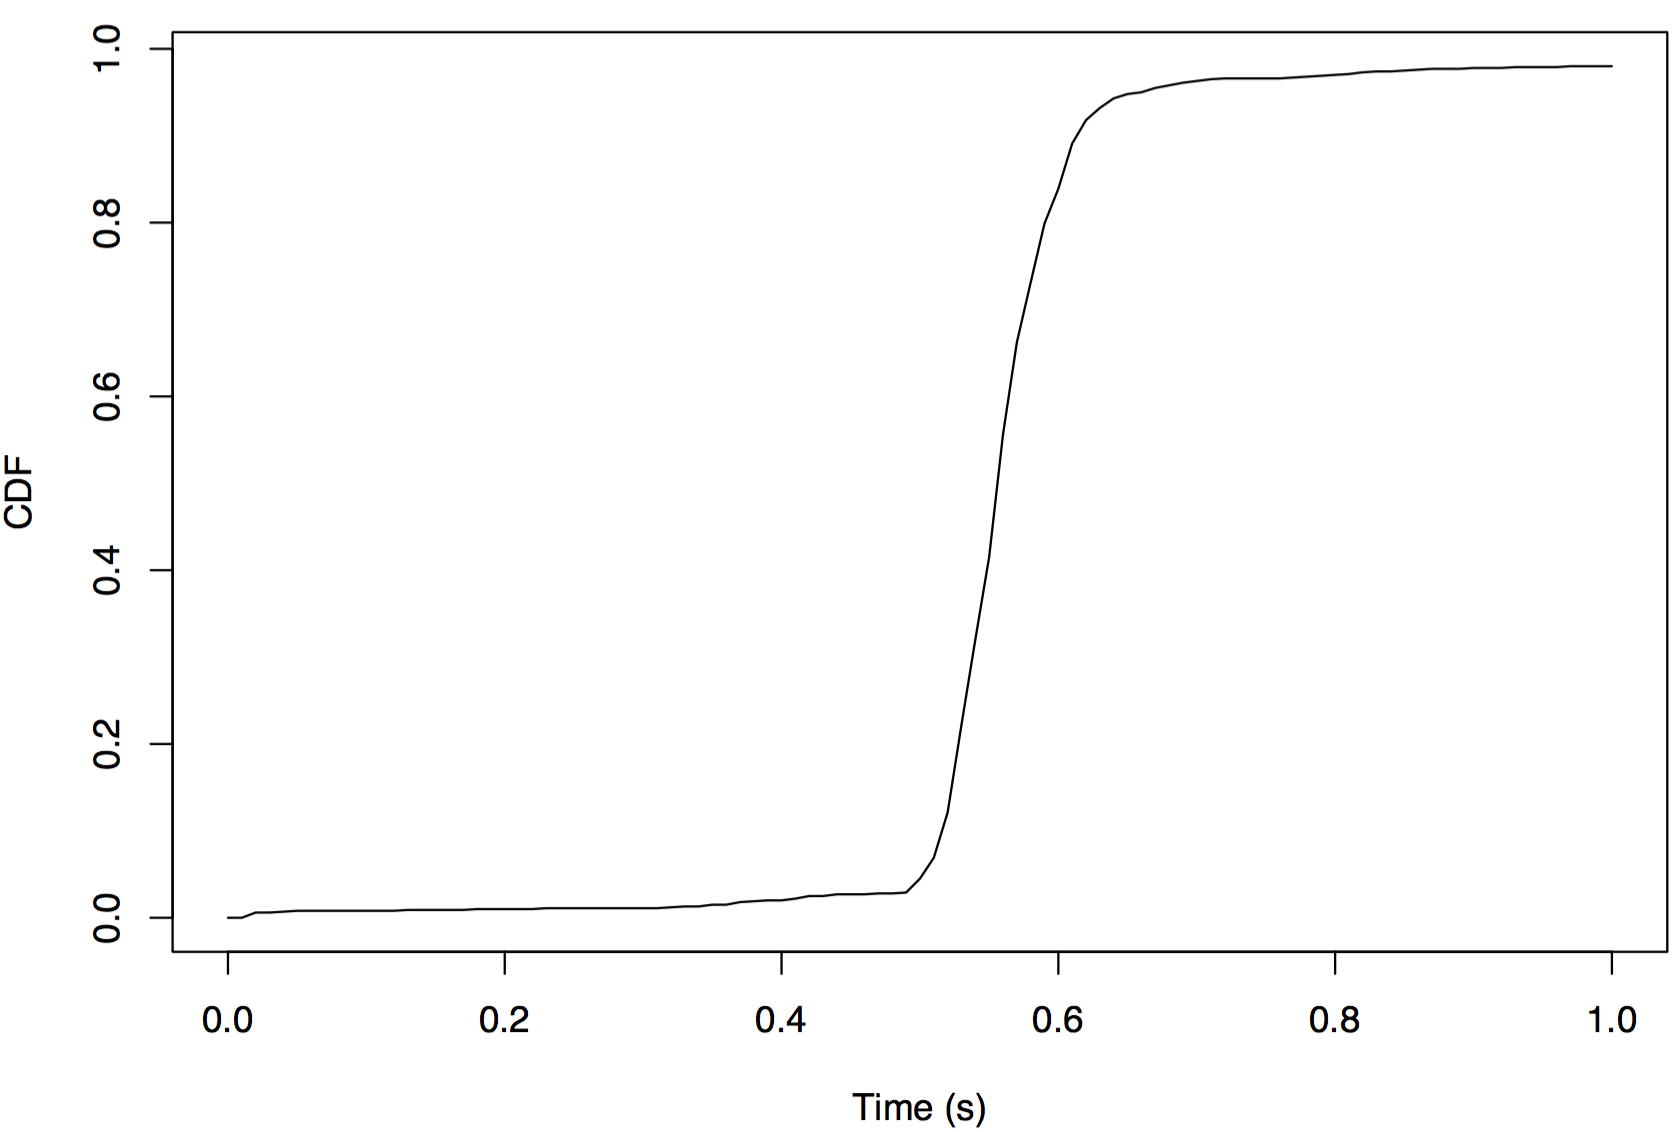
\includegraphics[width=80mm]{figure/runtime}
%\caption{Runtime of AS resilience calculation from a given source AS \label{fig_ascal}}
%\end{figure}

Next, we installed our new Tor client on $26$ Planetlab nodes located in different ASes, and performed page loads of Alexa top 100 websites. We compared the performance of $\alpha=\{0.25,0.5\}$ with $g=10\%$ random sampling against vanilla Tor. Figure ~\ref{fig_pageload} shows the page load time. We can see that all three have very similar performance. This can be explained in the following ways. First, we do not restrict the relay selection to a smaller set of relays, but rather \emph{preferring} certain relays over the others; second, the $\alpha$ value was tuned to be $\{0.25,0.5\}$, which gives sufficient weight to the bandwidth in relay selection; thirdly, the relay selected has a relatively short AS path (and is likely geographically closer);finally, the algorithm is only for guard relay selection, whereas exit relay selection remains the same as purely bandwidth-weighted selection. These are some reasons why the new guard relay selection algorithm does not suffer any performance loss in page load time. 

\begin{figure}[ht!]
\centering
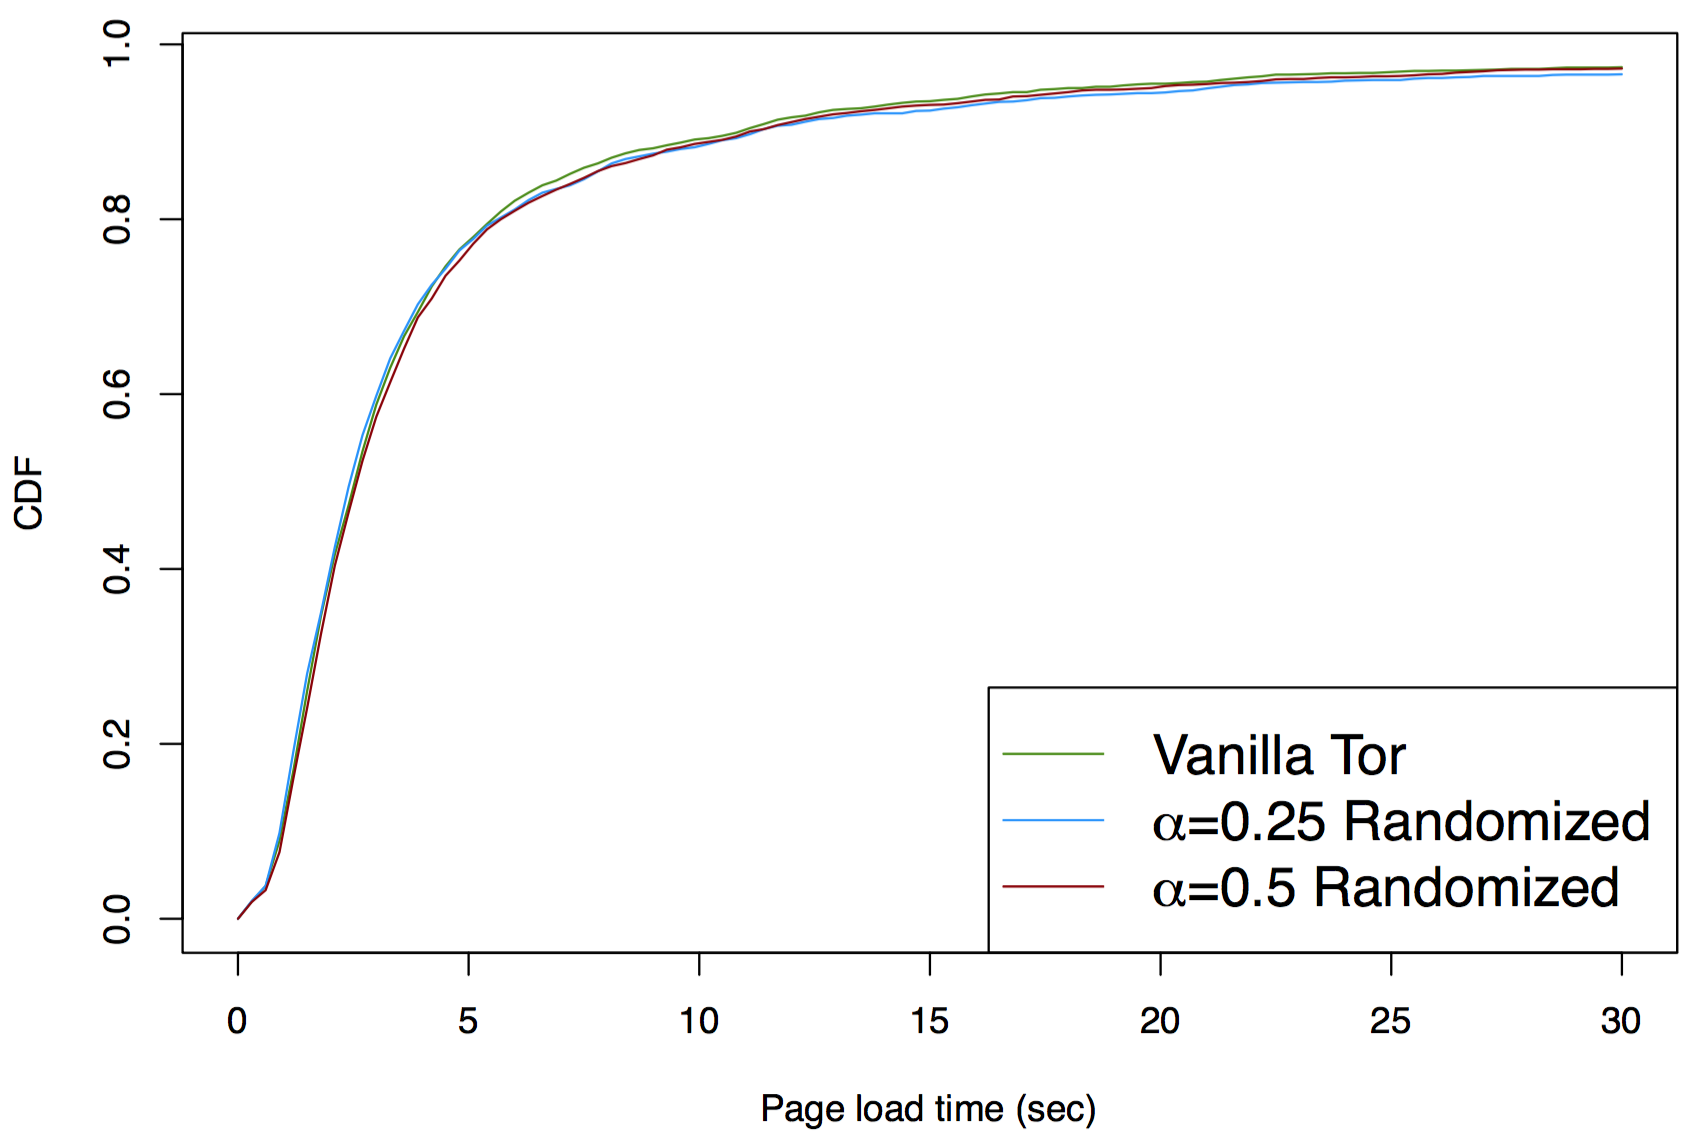
\includegraphics[width=80mm]{figure/pageloadtime}
\caption{Page load time of Alexa top 100 sites \label{fig_pageload}}
\end{figure}



